%% (Master) Thesis template
% Template version used: v1.4
%
% Largely adapted from Adrian Nievergelt's template for the ADPS
% (lecture notes) project.


%% We use the memoir class because it offers a many easy to use features.
\documentclass[11pt,a4paper,titlepage]{memoir}

%% Packages
%% ========

%% LaTeX Font encoding -- DO NOT CHANGE
\usepackage[OT1]{fontenc}

%% Babel provides support for languages.  'english' uses British
%% English hyphenation and text snippets like "Figure" and
%% "Theorem". Use the option 'ngerman' if your document is in German.
%% Use 'american' for American English.  Note that if you change this,
%% the next LaTeX run may show spurious errors.  Simply run it again.
%% If they persist, remove the .aux file and try again.
\usepackage[english]{babel}

%% Input encoding 'utf8'. In some cases you might need 'utf8x' for
%% extra symbols. Not all editors, especially on Windows, are UTF-8
%% capable, so you may want to use 'latin1' instead.
\usepackage[utf8]{inputenc}

%% This changes default fonts for both text and math mode to use Herman Zapfs
%% excellent Palatino font.  Do not change this.
\usepackage[sc]{mathpazo}

%% The AMS-LaTeX extensions for mathematical typesetting.  Do not
%% remove.
\usepackage{amsmath,amssymb,amsfonts,mathrsfs}

%% NTheorem is a reimplementation of the AMS Theorem package. This
%% will allow us to typeset theorems like examples, proofs and
%% similar.  Do not remove.
%% NOTE: Must be loaded AFTER amsmath, or the \qed placement will
%% break
\usepackage[amsmath,thmmarks]{ntheorem}

%% LaTeX' own graphics handling
\usepackage{graphicx}

%% We unfortunately need this for the Rules chapter.  Remove it
%% afterwards; or at least NEVER use its underlining features.
\usepackage{soul}

%% This allows you to add .pdf files. It is used to add the
%% declaration of originality.
\usepackage{pdfpages}

%% Some more packages that you may want to use.  Have a look at the
%% file, and consult the package docs for each.
%% See the TeXed file for more explanations

%% [OPT] Multi-rowed cells in tabulars
%\usepackage{multirow}

%% [REC] Intelligent cross reference package. This allows for nice
%% combined references that include the reference and a hint to where
%% to look for it.
\usepackage{varioref}

%% [OPT] Easily changeable quotes with \enquote{Text}
%\usepackage[german=swiss]{csquotes}

%% [REC] Format dates and time depending on locale
\usepackage{datetime}

%% [OPT] Provides a \cancel{} command to stroke through mathematics.
%\usepackage{cancel}

%% [NEED] This allows for additional typesetting tools in mathmode.
%% See its excellent documentation.
\usepackage{mathtools}

%% [ADV] Conditional commands
%\usepackage{ifthen}

%% [OPT] Manual large braces or other delimiters.
%\usepackage{bigdelim, bigstrut}

%% [REC] Alternate vector arrows. Use the command \vv{} to get scaled
%% vector arrows.
\usepackage[h]{esvect}

%% [NEED] Some extensions to tabulars and array environments.
\usepackage{array}

%% [OPT] Postscript support via pstricks graphics package. Very
%% diverse applications.
%\usepackage{pstricks,pst-all}

%% [?] This seems to allow us to define some additional counters.
%\usepackage{etex}

%% [ADV] XY-Pic to typeset some matrix-style graphics
%\usepackage[all]{xy}

%% [OPT] This is needed to generate an index at the end of the
%% document.
%\usepackage{makeidx}

%% [OPT] Fancy package for source code listings.  The template text
%% needs it for some LaTeX snippets; remove/adapt the \lstset when you
%% remove the template content.
\usepackage{listings}
\lstset{language=TeX,basicstyle={\normalfont\ttfamily}}

%% [REC] Fancy character protrusion.  Must be loaded after all fonts.
%% Must be outdated, see https://texwelt.de/fragen/27171/latex-error-command-ifpdftex-already-defined
% \usepackage[activate]{pdfcprot}

%% [REC] Nicer tables.  Read the excellent documentation.
\usepackage{booktabs}

\usepackage{natbib}

\usepackage{textgreek}

\usepackage{caption}

\usepackage{subcaption}

\usepackage{mleftright}     % proper spacing in maths mode

\usepackage{xspace}         % the eater of spaces

\usepackage{siunitx}


%% Our layout configuration.  DO NOT CHANGE.
%% Memoir layout setup

%% NOTE: You are strongly advised not to change any of them unless you
%% know what you are doing.  These settings strongly interact in the
%% final look of the document.

% Dependencies
\usepackage{ETHlogo}

\nonzeroparskip
\parindent=0pt
\defaultlists

% Chapter style redefinition
\makeatletter

\if@twoside
  \pagestyle{Ruled}
  \copypagestyle{chapter}{Ruled}
\else
  \pagestyle{ruled}
  \copypagestyle{chapter}{ruled}
\fi
\makeoddhead{chapter}{}{}{}
\makeevenhead{chapter}{}{}{}
\makeheadrule{chapter}{\textwidth}{0pt}
\copypagestyle{abstract}{empty}

\makechapterstyle{bianchimod}{%
  \chapterstyle{default}
  \renewcommand*{\chapnamefont}{\normalfont\Large}
  \renewcommand*{\chapnumfont}{\normalfont\Large}
  \renewcommand*{\printchaptername}{%
    \chapnamefont\centering\@chapapp}
  \renewcommand*{\printchapternum}{\chapnumfont {\thechapter}}
  \renewcommand*{\chaptitlefont}{\normalfont\huge}
  \renewcommand*{\printchaptertitle}[1]{%
    \hrule\vskip\onelineskip \centering \chaptitlefont\textbf{\vphantom{gyM}##1}\par}
  \renewcommand*{\afterchaptertitle}{\vskip\onelineskip \hrule\vskip
    \afterchapskip}
  \renewcommand*{\printchapternonum}{%
    \vphantom{\chapnumfont {9}}\afterchapternum}}

% Use the newly defined style
\chapterstyle{bianchimod}

\setsecheadstyle{\Large\bfseries}
\setsubsecheadstyle{\large\bfseries}
\setsubsubsecheadstyle{\bfseries}
\setparaheadstyle{\normalsize\bfseries}
\setsubparaheadstyle{\normalsize\itshape}
\setsubparaindent{0pt}

% Set captions to a more separated style for clearness
\captionnamefont{\bfseries\footnotesize}
\captiontitlefont{\footnotesize}
\setlength{\intextsep}{16pt}
\setlength{\belowcaptionskip}{1pt}

% Set section and TOC numbering depth to subsection
\setsecnumdepth{subsection}
\settocdepth{subsection}

%% Titlepage adjustments
\pretitle{\vspace{0pt plus 0.7fill}\begin{center}\HUGE\bfseries}
\posttitle{\end{center}\par}
\preauthor{\par\begin{center}\let\and\\\Large}
\postauthor{\end{center}}
\predate{\par\begin{center}\Large}
\postdate{\end{center}}

\def\@advisors{}
\newcommand{\advisors}[1]{\def\@advisors{#1}}
\def\@department{}
\newcommand{\department}[1]{\def\@department{#1}}
\def\@thesistype{}
\newcommand{\thesistype}[1]{\def\@thesistype{#1}}

\renewcommand{\maketitlehooka}{\noindent\ETHlogo[2in]}

\renewcommand{\maketitlehookb}{\vspace{1in}%
  \par\begin{center}\Large\@thesistype\end{center}}

\renewcommand{\maketitlehookd}{%
  \vfill\par
  \begin{flushright}
    \@advisors\par
    \@department, ETH Z\"urich
  \end{flushright}
}
% Set same size of margins
\setlrmargins{*}{*}{1}
\checkandfixthelayout

% \setlength{\droptitle}{-48pt}

% Turn extra space before chapter headings off.
\setlength{\beforechapskip}{0pt}

\makeatother

% This defines how theorems should look. Best leave as is.
\theoremstyle{plain}
\setlength\theorempostskipamount{0pt}

%%% Local Variables:
%%% mode: latex
%%% TeX-master: "thesis"
%%% End:


%% Theorem environments.  You will have to adapt this for a German
%% thesis.
%% Theorem-like environments

%% This can be changed according to language. You can comment out the ones you
%% don't need.

\numberwithin{equation}{chapter}

%% German theorems
%\newtheorem{satz}{Satz}[chapter]
%\newtheorem{beispiel}[satz]{Beispiel}
%\newtheorem{bemerkung}[satz]{Bemerkung}
%\newtheorem{korrolar}[satz]{Korrolar}
%\newtheorem{definition}[satz]{Definition}
%\newtheorem{lemma}[satz]{Lemma}
%\newtheorem{proposition}[satz]{Proposition}

%% English variants
\newtheorem{theorem}{Theorem}[chapter]
\newtheorem{example}[theorem]{Example}
\newtheorem{remark}[theorem]{Remark}
\newtheorem{corollary}[theorem]{Corollary}
\newtheorem{definition}[theorem]{Definition}
\newtheorem{lemma}[theorem]{Lemma}
\newtheorem{proposition}[theorem]{Proposition}

%% Proof environment with a small square as a "qed" symbol
\theoremstyle{nonumberplain}
\theorembodyfont{\normalfont}
\theoremsymbol{\ensuremath{\square}}
\newtheorem{proof}{Proof}
%\newtheorem{beweis}{Beweis}


%% Helpful macros.
%% Custom commands
%% ===============

%% Special characters for number sets, e.g. real or complex numbers.
\newcommand{\C}{\mathbb{C}}
\newcommand{\K}{\mathbb{K}}
\newcommand{\N}{\mathbb{N}}
\newcommand{\Q}{\mathbb{Q}}
\newcommand{\R}{\mathbb{R}}
\newcommand{\Z}{\mathbb{Z}}
\newcommand{\X}{\mathbb{X}}

%% Fixed/scaling delimiter examples (see mathtools documentation)
\DeclarePairedDelimiter\abs{\lvert}{\rvert}
\DeclarePairedDelimiter\norm{\lVert}{\rVert}

%% Use the alternative epsilon per default and define the old one as \oldepsilon
\let\oldepsilon\epsilon
\renewcommand{\epsilon}{\ensuremath\varepsilon}

%% Also set the alternate phi as default.
\let\oldphi\phi
\renewcommand{\phi}{\ensuremath{\varphi}}

%% Some macros useful for this thesis
\newcommand{\tk}{\text{k}} % kernel function
\newcommand{\td}{\text{d}} % distance function
\newcommand{\MMD}{\text{MMD}} % distance function
\newcommand{\bx}{\mathbf{x}} % distance function
\newcommand{\by}{\mathbf{y}} % distance function

\interfootnotelinepenalty=10000


%% Make document internal hyperlinks wherever possible. (TOC, references)
%% This MUST be loaded after varioref, which is loaded in 'extrapackages'
%% above.  We just load it last to be safe.
\usepackage[linkcolor=black,colorlinks=true,citecolor=black,filecolor=black]{hyperref}


%% Document information
%% ====================

\title{Title of Thesis}
\author{S. Tudent}
\thesistype{Master Thesis}
\advisors{Advisors: Prof.\ Dr.\ A. D. Visor, Dr.\ P. Ostdoc}
\department{Department of Computer Science}
\date{January 19, 2038}

\begin{document}

\frontmatter

%% Title page is autogenerated from document information above.  DO
%% NOT CHANGE.
\begin{titlingpage}
  \calccentering{\unitlength}
  \begin{adjustwidth*}{\unitlength-24pt}{-\unitlength-24pt}
    \maketitle
  \end{adjustwidth*}
\end{titlingpage}

%% The abstract of your thesis.  Edit the file as needed.
\begin{abstract}
Generative models applied proteins are poised to revolutionize the \emph{in
silico} design of novel proteins satisfying various functional and shape-related
constraints. However, such models are hard to evaluate -- determining how
realistic a generated set of proteins is represents one of the major challenges
in the field of generative models applied to proteins. For graphs, a
representation often used to investigate proteins, the community has gravitated
toward using a kernel two-sample test statistic called the maximum mean
discrepancy. While recent works highlighted some of its pitfalls, this statistic
remains highly versatile since any kernel can be used.

In this thesis, we start by evaluating the expressivity, robustness and
efficiency of maximum mean discrepancy on graph descriptors using graphs
directly extracted from proteins. We then expand the use of MMD by using novel
representations, descriptor functions, and kernels. Specifically, we investigate
the use of graph kernels in MMD. We also devise and apply novel protein-specific
descriptors, such as the dihedral angles histogram formed by each amino acid,
and the pairwise distance histogram of each amino acid, which are both highly
expressive and effecient. Finally, we apply a class of kernels able to operate
on persistence diagrams, a powerful topological descriptor leveraging the
shape-related information in the point clouds formed by each protein structure.


\end{abstract}


%% TOC with the proper setup, do not change.
\cleartorecto
\tableofcontents
\mainmatter

%% Your real content!
\chapter{Introduction}

% Target length: 1,5 pages.

Generative modelling is a highly active branch of machine learning aiming to
model the joint distribution of a certain feature set $x$ and target labels $y$,
often referred to as $p(x,y)$. Modelling this joint distribution presents a lot
of advantages in a myriad of domains, but can be especially
consequential in biology \citep{lopez2020enhancing,strokach2022deep}.

In protein science specifically, the application domains of generative models
can solve a myriad of relevant tasks, from novel protein sequence design, to
designing proteins with specific shapes or functions
\citep{jendrusch2021alphadesign,madani2021deep}. Moreover, the resulting models generate
embeddings and/or weights which can be transferred to discriminative settings
where one seeks to predict $y$ given $x$, i.e. $p(y|x)$. In such a setting, even
more tasks can be tackled using generative models as a starting point, such as protein
structure prediction \citep{jumper2021highly}, function prediction
\citep{meier2021language}, stability prediction \citep{strokach2020fast}.

However, the design and improvement of generative model designs applied to
proteins is prohibited by the lack of suitable evaluation metrics. It is
notoriously hard to find expressive, robust and efficient performance measures
that accurately gauge the quality of generated samples. Efforts have been
made to solve this challenge in the image domain \citep{heusel2017gans}, and
recently, the community has investigated this challenge specifically for a
common representation of proteins: graphs \citep{thompson2022evaluation,
 obray2022evaluation}. In this domain, the standard measure used is a highly
versatile statistic for a kernel two-sample test called \acrfull{mmd}
\citep{gretton2012kernel}.

The results of these investigations, especially those conducted by
\cite{obray2022evaluation}, unveiled a number of pitfalls related to \acrshort{mmd}. Depending
on the kernel and kernel parameter configuration, different \acrshort{mmd} configurations
ranked the quality of samples generated by different models differently. In
addition, when progressively perturbing a set of synthetic graphs, certain \acrshort{mmd}
configurations with respect to another set of unperturbed graphs issued from the
same distribution was not always found to monotonically increase with increasing
amounts of perturbations, casting doubt on the expressivity of \acrshort{mmd} in certain
configurations and data.

In this thesis, we set out to clarify the behaviour of various \acrshort{mmd}
configurations on protein data sets and perform a meta-evaluation of \acrshort{mmd}-based
metrics. We investigate the behaviour of various \acrshort{mmd} configurations by applying
perturbations to one set of proteins. These perturbations are relevant for
protein design use cases and include sequence perturbations, graph perturbations
and geometric perturbations. In this setting, we investigate the behaviour of
classical \acrshort{mmd} configurations typically used to evaluate generative models in the
graph domain. In addition, we expand this set of configurations by devising
novel combinations of protein representations, descriptors, and kernels, all
relevant for different aspects of protein design, and integrate them to the
well-established \acrshort{mmd} evaluation framework.

This thesis is organized as follows: first, Chapter \ref{chap:background}
introduces fundamental concepts that we are going to build upon, and discusses
the surrounding literature. Chapter \ref{chap:methods} details the methodology
of the various experiments that we carry out in this thesis, as well as
describes all the configurations of \acrshort{mmd} that we will explore (i.e. all
combinations of representations, descriptor functions, kernels, and kernel
parameters). Chapter \ref{chap:results} presents and contextualizes the findings of those
experiments. We summarize key findings, make recommendations for practitioners and
highlight some limitations and directions for future work in Chapter
\ref{chap:discussion} before concluding in Chapter \ref{chap:conclusion}.

% Graph representations encapsulates a wide variety of data. Show how they can
% be useful in biology.

% Leslie paper: even worse, depending on parametrization, different models come
% out on top. Call for principled metric design is open.

% Machine learning for graphs. Describe different tasks. Discriminative vs.
% generative modelling.

% Challenges with generative modelling assessment, especially with related to
% graphs vs images. Situate within proteins. Show that it builds on Obray et al.

% Thesis overview

\chapter{Writing scientific texts in English}

This chapter was originally a separate document written by Reto
Spöhel.  It is reprinted here so that the template can serve as a
quick guide to thesis writing, and to provide some more example
material to give you a feeling for good typesetting.

% We're going to need an extra theorem-like environment for this
% chapter
\theoremstyle{plain}
\theoremsymbol{}
\newtheorem{Rule}[theorem]{Rule}

\section{Basic writing rules}

The following rules need little further explanation; they are best
understood by looking at the example in the booklet by Knuth et al.,
§2--§3.

\begin{Rule}
  Write texts, not chains of formulas.
\end{Rule}

More specifically, write full sentences that are logically
interconnected by phrases like `Therefore', `However', `On the other
hand', etc.\ where appropriate.

\begin{Rule}
  Displayed formulas should be embedded in your text and punctuated
  with it.
\end{Rule}

In other words, your writing should not be divided into `text parts'
and `formula parts'; instead the formulas should be tied together by
your prose such that there is a natural flow to your writing.

\section{Being nice to the reader}

Try to write your text in such a way that a reader enjoys reading
it. That's of course a lofty goal, but nevertheless one you should
aspire to!

\begin{Rule}
  Be nice to the reader.
\end{Rule}

Give some intuition or easy example for definitions and theorems which
might be hard to digest. Remind the reader of notations you introduced
many pages ago -- chances are he has forgotten them. Illustrate your
writing with diagrams and pictures where this helps the reader. Etc.

\begin{Rule}
  Organize your writing.
\end{Rule}

Think carefully about how you subdivide your thesis into chapters,
sections, and possibly subsections.  Give overviews at the beginning
of your thesis and of each chapter, so the reader knows what to
expect. In proofs, outline the main ideas before going into technical
details. Give the reader the opportunity to `catch up with you' by
summing up your findings periodically.

\emph{Useful phrases:} `So far we have shown that \ldots', `It remains
to show that \ldots', `Recall that we want to prove inequality (7), as
this will allow us to deduce that \ldots', `Thus we can conclude that
\ldots. Next, we would like to find out whether \ldots', etc.

\begin{Rule}
  Don't say the same thing twice without telling the reader that you
  are saying it twice.
\end{Rule}

Repetition of key ideas is important and helpful. However, if you
present the same idea, definition or observation twice (in the same or
different words) without telling the reader, he will be looking for
something new where there is nothing new.

\emph{Useful phrases:} `Recall that [we have seen in Chapter 5 that]
\ldots', `As argued before / in the proof of Lemma 3, \ldots', `As
mentioned in the introduction, \ldots', `In other words, \ldots', etc.

\begin{Rule}
  Don't make statements that you will justify later without telling
  the reader that you will justify them later.
\end{Rule}

This rule also applies when the justification is coming right in the
next sentence!  The reasoning should be clear: if you violate it, the
reader will lose valuable time trying to figure out on his own what
you were going to explain to him anyway.

\emph{Useful phrases:} `Next we argue that \ldots', `As we shall see,
\ldots', `We will see in the next section that \ldots, etc.


\section{A few important grammar rules}

\begin{Rule}
  \label{rule:no-comma-before-that}
  There is (almost) \emph{never} a comma before `that'.
\end{Rule}

It's really that simple. Examples:
\begin{quote}
  We assume that \ldots\\
  \emph{Wir nehmen an, dass \ldots}

  It follows that \ldots\\
  \emph{Daraus folgt, dass \ldots}

  `thrice' is a word that is seldom used.\\
  \emph{`thrice' ist ein Wort, das selten verwendet wird.}
\end{quote}
Exceptions to this rule are rare and usually pretty obvious. For
example, you may end up with a comma before `that' because `i.e.' is
spelled out as `that is':
\begin{quote}
  For \(p(n)=\log n/n\) we have \ldots{} However, if we choose \(p\) a
  little bit higher, that is \(p(n)=(1+\varepsilon)\log n/n\) for some
  \(\varepsilon>0\), we obtain that\ldots
\end{quote}
Or you may get a comma before `that' because there is some additional
information inserted in the middle of your sentence:
\begin{quote}
  Thus we found a number, namely \(n_0\), that satisfies equation (13).
\end{quote}
If the additional information is left out, the sentence has no comma:
\begin{quote}
  Thus we found a number that satisfies equation (13).
\end{quote}
(For `that' as a relative pronoun, see also
Rules~\ref{rule:non-defining-has-comma}
and~\ref{rule:defining-without-comma} below.)

\begin{Rule}
  There is usually no comma before `if'.
\end{Rule}

Example:
\begin{quote}
  A graph is not \(3\)-colorable if it contains a \(4\)-clique.\\
  \emph{Ein Graph ist nicht \(3\)-färbbar, wenn er eine \(4\)-Clique
    enthält.}
\end{quote}
However, if the `if' clause comes first, it is usually separated from
the main clause by a comma:
\begin{quote}
  If a graph contains a \(4\)-clique, it is not \(3\)-colorable .\\
  \emph{Wenn ein Graph eine \(4\)-Clique enthält, ist er nicht
    \(3\)-färbbar.}
\end{quote}

There are more exceptions to these rules than to
Rule~\ref{rule:no-comma-before-that}, which is why we are not
discussing them here. Just keep in mind: don't put a comma before `if'
without good reason.

\begin{Rule}
  \label{rule:non-defining-has-comma}
  Non-defining relative clauses have commas.
\end{Rule}
\begin{Rule}
  \label{rule:defining-without-comma}
  Defining relative clauses have no commas.
\end{Rule}

In English, it is very important to distinguish between two types of
relative clauses: defining and non-defining ones. This is a
distinction you absolutely need to understand to write scientific
texts, because mistakes in this area actually distort the meaning of
your text!

It's probably easier to explain first what a \emph{non-defining}
relative clause is. A non-defining relative clauses simply gives
additional information \emph{that could also be left out} (or given in
a separate sentence). For example, the sentence
\begin{quote}
  The \textsc{WeirdSort} algorithm, which was found by the famous
  mathematician John Doe, is theoretically best possible but difficult
  to implement in practice.
\end{quote}
would be fully understandable if the relative clause were left out
completely. It could also be rephrased as two separate sentences:
\begin{quote}
  The \textsc{WeirdSort} algorithm is theoretically best possible but
  difficult to implement in practice. [By the way,] \textsc{WeirdSort}
  was found by the famous mathematician John Doe.
\end{quote}
This is what a non-defining relative clause is. \emph{Non-defining
  relative clauses are always written with commas.} As a corollary we
obtain that you cannot use `that' in non-defining relative clauses
(see Rule~\ref{rule:no-comma-before-that}!). It would be wrong to
write
\begin{quote}
  \st{The \textsc{WeirdSort} algorithm, that was found by the famous
    mathematician John Doe, is theoretically best possible but
    difficult to implement in practice.}
\end{quote}
A special case that warrants its own example is when `which' is
referring to the entire preceding sentence:
\begin{quote}
  Thus inequality (7) is true, which implies that the Riemann
  hypothesis holds.
\end{quote}
As before, this is a non-defining relative sentence (it could be left
out) and therefore needs a comma.

So let's discuss \emph{defining} relative clauses next. A defining
relative clause tells the reader \emph{which specific item the main
  clause is talking about}. Leaving it out either changes the meaning
of the sentence or renders it incomprehensible altogether.  Consider
the following example:

\begin{quote}
  The \textsc{WeirdSort} algorithm is difficult to implement in
  practice. In contrast, the algorithm that we suggest is very simple.
\end{quote}

Here the relative clause `that we suggest' cannot be left out -- the
remaining sentence would make no sense since the reader would not know
which algorithm it is talking about. This is what a defining relative
clause is. \textit{Defining relative clauses are never written with
  commas.} Usually, you can use both `that' and `which' in defining
relative clauses, although in many cases `that' sounds better.

As a final example, consider the following sentence:
\begin{quote}
  For the elements in \(\mathcal{B}\) which satisfy property (A), we
  know that equation (37) holds.
\end{quote}
This sentence does not make a statement about all elements in
\(\mathcal{B}\), only about those satisfying property (A). The relative
clause is \emph{defining}. (Thus we could also use `that' in place of
`which'.)

In contrast, if we add a comma the sentence reads
\begin{quote}
  For the elements in \(\mathcal{B}\), which satisfy property (A), we
  know that equation (37) holds.
\end{quote}

Now the relative clause is \emph{non-defining} -- it just mentions in
passing that all elements in \(\mathcal{B}\) satisfy property (A). The
main clause states that equation (37) holds for \emph{all} elements in
\(\mathcal{B}\). See the difference?


\section[Things you (usually) don't say in English]%
{Things you (usually) don't say in English -- and what to say
  instead}
\label{sec:list}

Table~\ref{tab:things-you-dont-say} lists some common mistakes and
alternatives.  The entries should not be taken as gospel -- they don't
necessarily mean that a given word or formulation is wrong under all
circumstances (obviously, this depends a lot on the context). However,
in nine out of ten instances the suggested alternative is the better
word to use.

\begin{table}
  \centering
  \caption{Things you (usually) don't say}
  \label{tab:things-you-dont-say}
  \begin{tabular}{lll}
    \toprule
    \st{It holds (that) \dots} & We have \dots & \emph{Es gilt \dots}\\
    \multicolumn{3}{l}{\quad\footnotesize(`Equation (5) holds.' is fine, though.)}\\
    \st{$x$ fulfills property $\mathcal{P}$.}& \(x\) satisfies property \(\mathcal{P}\). & \emph{\(x\) erfüllt Eigenschaft \(\mathcal{P}\).} \\
    \st{in average} & on average & \emph{im Durchschnitt}\\
    \st{estimation} & estimate   & \emph{Abschätzung}\\
    \st{composed number} & composite number & \emph{zusammengesetzte Zahl}\\
    \st{with the help of} & using & \emph{mit Hilfe von}\\
    \st{surely} & clearly & \emph{sicher, bestimmt}\\
    \st{monotonously increasing} & monotonically incr. & \emph{monoton steigend}\\
    \multicolumn{3}{l}{\quad\footnotesize(Actually, in most cases `increasing' is just fine.)}\\
    \bottomrule
  \end{tabular}
\end{table}

%%% Local Variables:
%%% mode: latex
%%% TeX-master: "thesis"
%%% End:

\chapter{Typography}


\section{Punctuation}

\begin{Rule}
  Use opening (`) and closing (') quotation marks correctly.
\end{Rule}

In \LaTeX, the closing quotation mark is typed like a normal
apostrophe, while the opening quotation mark is typed using the French
\emph{accent grave} on your keyboard (the \emph{accent grave} is the
one going down, as in \emph{frère}).

Note that any punctuation that \emph{semantically} follows quoted
speech goes inside the quotes in American English, but outside in
Britain.  Also, Americans use double quotes first.  Oppose
\begin{quote}
  ``Using `lasers,' we punch a hole in \ldots\ the Ozone Layer,''
  Dr.\ Evil said.
\end{quote}
to
\begin{quote}
  `Using ``lasers'', we punch a hole in \ldots\ the Ozone Layer',
  Dr.\ Evil said.
\end{quote}

\begin{Rule}
  Use hyphens (-), en-dashes (--) and em-dashes (---) correctly.
\end{Rule}

A hyphen is only used in words like `well-known', `$3$-colorable'
etc., or to separate words that continue in the next line (which is
known as hyphenation).  It is entered as a single ASCII hyphen
character (\texttt{-}).

To denote ranges of numbers, chapters, etc., use an en-dash (entered
as two ASCII hyphens \texttt{--}) with no spaces on either side.  For
example, using Equations (1)--(3), we see\ldots

As the equivalent of the German \emph{Gedankenstrich}, use an en-dash
with spaces on both sides -- in the title of Section \ref{sec:list},
it would be wrong to use a hyphen instead of the dash. (Some English
authors use the even longer emdash (---) instead, which is typed as
three subsequent hyphens in \LaTeX. This emdash is used without spaces
around it---like so.)


\section{Spacing}

\begin{Rule}
  \label{rule:no-manual-spacing}
  Do not add spacing manually.
\end{Rule}

You should never use the commands \lstinline-\\- (except within
tabulars and arrays), \lstinline[showspaces=true]-\ - (except to
prevent a sentence-ending space after Dr.\ and such),
\lstinline-\vspace-, \lstinline-\hspace-, etc.  The choices programmed
into \LaTeX{} and this style should cover almost all cases.  Doing it
manually quickly leads to inconsistent spacing, which looks terrible.
Note that this list of commands is by no means conclusive.

\begin{Rule}
  Judiciously insert spacing in maths where it helps.
\end{Rule}

This directly contradicts Rule~\ref{rule:no-manual-spacing}, but in
some cases \TeX{} fails to correctly decide how much spacing is
required.  For example, consider
\begin{displaymath}
  f(a,b) = f(a+b, a-b).
\end{displaymath}
In such cases, inserting a thin math space \lstinline-\,- greatly
increases readability:
\begin{displaymath}
  f(a,b) = f(a+b,\, a-b).
\end{displaymath}

Along similar lines, there are variations of some symbols with
different spacing.  For example, Lagrange's Theorem states that
\(\abs{G}=[G:H]\abs{H}\), but the proof uses a bijection \(f\colon
aH\to bH\).  (Note how the first colon is symmetrically spaced, but
the second is not.)

\begin{Rule}
  Learn when to use \lstinline[showspaces=true]-\ - and
  \lstinline-\@-.
\end{Rule}

Unless you use `french spacing', the space at the end of a sentence is
slightly larger than the normal interword space.

The rule used by \TeX{} is that any space following a period,
exclamation mark or question mark is sentence-ending, except for
periods preceded by an upper-case letter.  Inserting \lstinline-\-
before a space turns it into an interword space, and inserting
\lstinline-\@- before a period makes it sentence-ending.  This means
you should write
\begin{lstlisting}
Prof.\ Dr.\ A. Steger is a member of CADMO\@.
If you want to write a thesis with her, you
should use this template.
\end{lstlisting}
which turns into
\begin{quote}
  Prof.\ Dr.\ A. Steger is a member of CADMO\@.  If you want to write
  a thesis with her, you should use this template.
\end{quote}
The effect becomes more dramatic in lines that are stretched slightly
during justification:
\begin{quote}
  \parbox{\linewidth}{\hbox to \linewidth{%
      Prof.\ Dr.\ A. Steger is a member of CADMO\@.  If you}}
\end{quote}

\begin{Rule}
  Place a non-breaking space (\lstinline-~-) right before references.
\end{Rule}

This is actually a slight simplification of the real rule, which
should invoke common sense.  Place non-breaking spaces where a line
break would look `funny' because it occurs right in the middle of a
construction, especially between a reference type (Chapter) and its
number.


\section{Choice of `fonts'}

Professional typography distinguishes many font attributes, such as
family, size, shape, and weight.  The choice for sectional divisions
and layout elements has been made, but you will still occasionally
want to switch to something else to get the reader's attention.  The
most important rule is very simple.

\begin{Rule}
  When emphasising a short bit of text, use \lstinline-\emph-.
\end{Rule}

In particular, \emph{never} use bold text (\lstinline-\textbf-).
Italics (or Roman type if used within italics) avoids distracting the
eye with the huge blobs of ink in the middle of the text that bold
text so quickly introduces.

Occasionally you will need more notation, for example, a consistent
typeface used to identify algorithms.

\begin{Rule}
  Vary one attribute at a time.
\end{Rule}

For example, for \textsc{WeirdSort} we only changed the shape to small
caps.  Changing two attributes, say, to bold small caps would be
excessive (\LaTeX{} does not even have this particular variation).
The same holds for mathematical notation: the reader can easily
distinguish \(g_n\), \(G(x)\), \(\mathcal{G}\) and \(\mathsf{G}\).

\begin{Rule}
  Never underline or uppercase.
\end{Rule}

No exceptions to this one, unless you are writing your thesis on a
typewriter.  Manually.  Uphill both ways.  In a blizzard.


\section{Displayed equations}

\begin{Rule}
  Insert paragraph breaks \emph{after} displays only where they
  belong.  Never insert paragraph breaks \emph{before} displays.
\end{Rule}

\LaTeX{} translates sequences of more than one linebreak (i.e., what
looks like an empty line in the source code) into a paragraph break in
almost all contexts.  This also happens before and after displays,
where extra spacing is inserted to give a visual indication of the
structure.  Adding a blank line in these places may look nice in the
sources, but compare the resulting display

\begin{displaymath}
  a = b
\end{displaymath}

to the following:
\begin{displaymath}
  a = b
\end{displaymath}
The first display is surrounded by blank lines, but the second is not.
It is bad style to start a paragraph with a display (you should always
tell the reader what the display means first), so the rule follows.

\begin{Rule}
  Never use \lstinline-eqnarray-.
\end{Rule}

It is at the root of most ill-spaced multiline displays.  The
\package{amsmath} package provides better alternatives, such as the
\lstinline-align- family
\begin{align*}
  f(x) &= \sin x, \\
  g(x) &= \cos x,
\end{align*}
and \lstinline-multline- which copes with excessively long equations:
\begin{multline*}
  \def\P{\mathrm P}
  \P\bigl[X_{t_0} \in (z_0, z_0+dz_0],\ldots, X_{t_n}\in(z_n,z_n+dz_n]\bigr]
  \\= \nu(dz_0) K_{t_1}(z_0,dz_1) K_{t_2-t_1}(z_1,dz_2)\cdots
  K_{t_n-t_{n-1}}(z_{n-1},dz_n).
\end{multline*}


\section{Floats}

By default this style provides floating environments for tables and
figures.  The general structure should be as follows:
\begin{lstlisting}
\begin{figure}
  \centering
  % content goes here
  \caption{A short caption}
  \label{some-short-label}
\end{figure}
\end{lstlisting}
Note that the label must follow the caption, otherwise the label will
refer to the surrounding section instead.  Also note that figures
should be captioned at the bottom, and tables at the top.

The whole point of floats is that they, well, \emph{float} to a place
where they fit without interrupting the text body.  This is a frequent
source of confusion and changes; please leave it as is.

\begin{Rule}
  Do not restrict float movement to only `here'
  \textnormal{(\lstinline-h-)}.
\end{Rule}

If you are still tempted, you should avoid the float altogether and
just show the figure or table inline, similar to a displayed equation.

%%% Local Variables:
%%% mode: latex
%%% TeX-master: "thesis"
%%% End:

\chapter{Example Chapter}

Dummy text.

\section{Example Section}

Dummy text.

\subsection{Example Subsection}

Dummy text.

\subsubsection{Example Subsubsection}

Dummy text.

\paragraph{Example Paragraph}

Dummy text.

\subparagraph{Example Subparagraph}

Dummy text.


\appendix

\chapter{Appendix}

\section{Influence of $k$ on sensitivity to perturbations of $k$-NN graphs}

\begin{figure}[h]
  \centering
  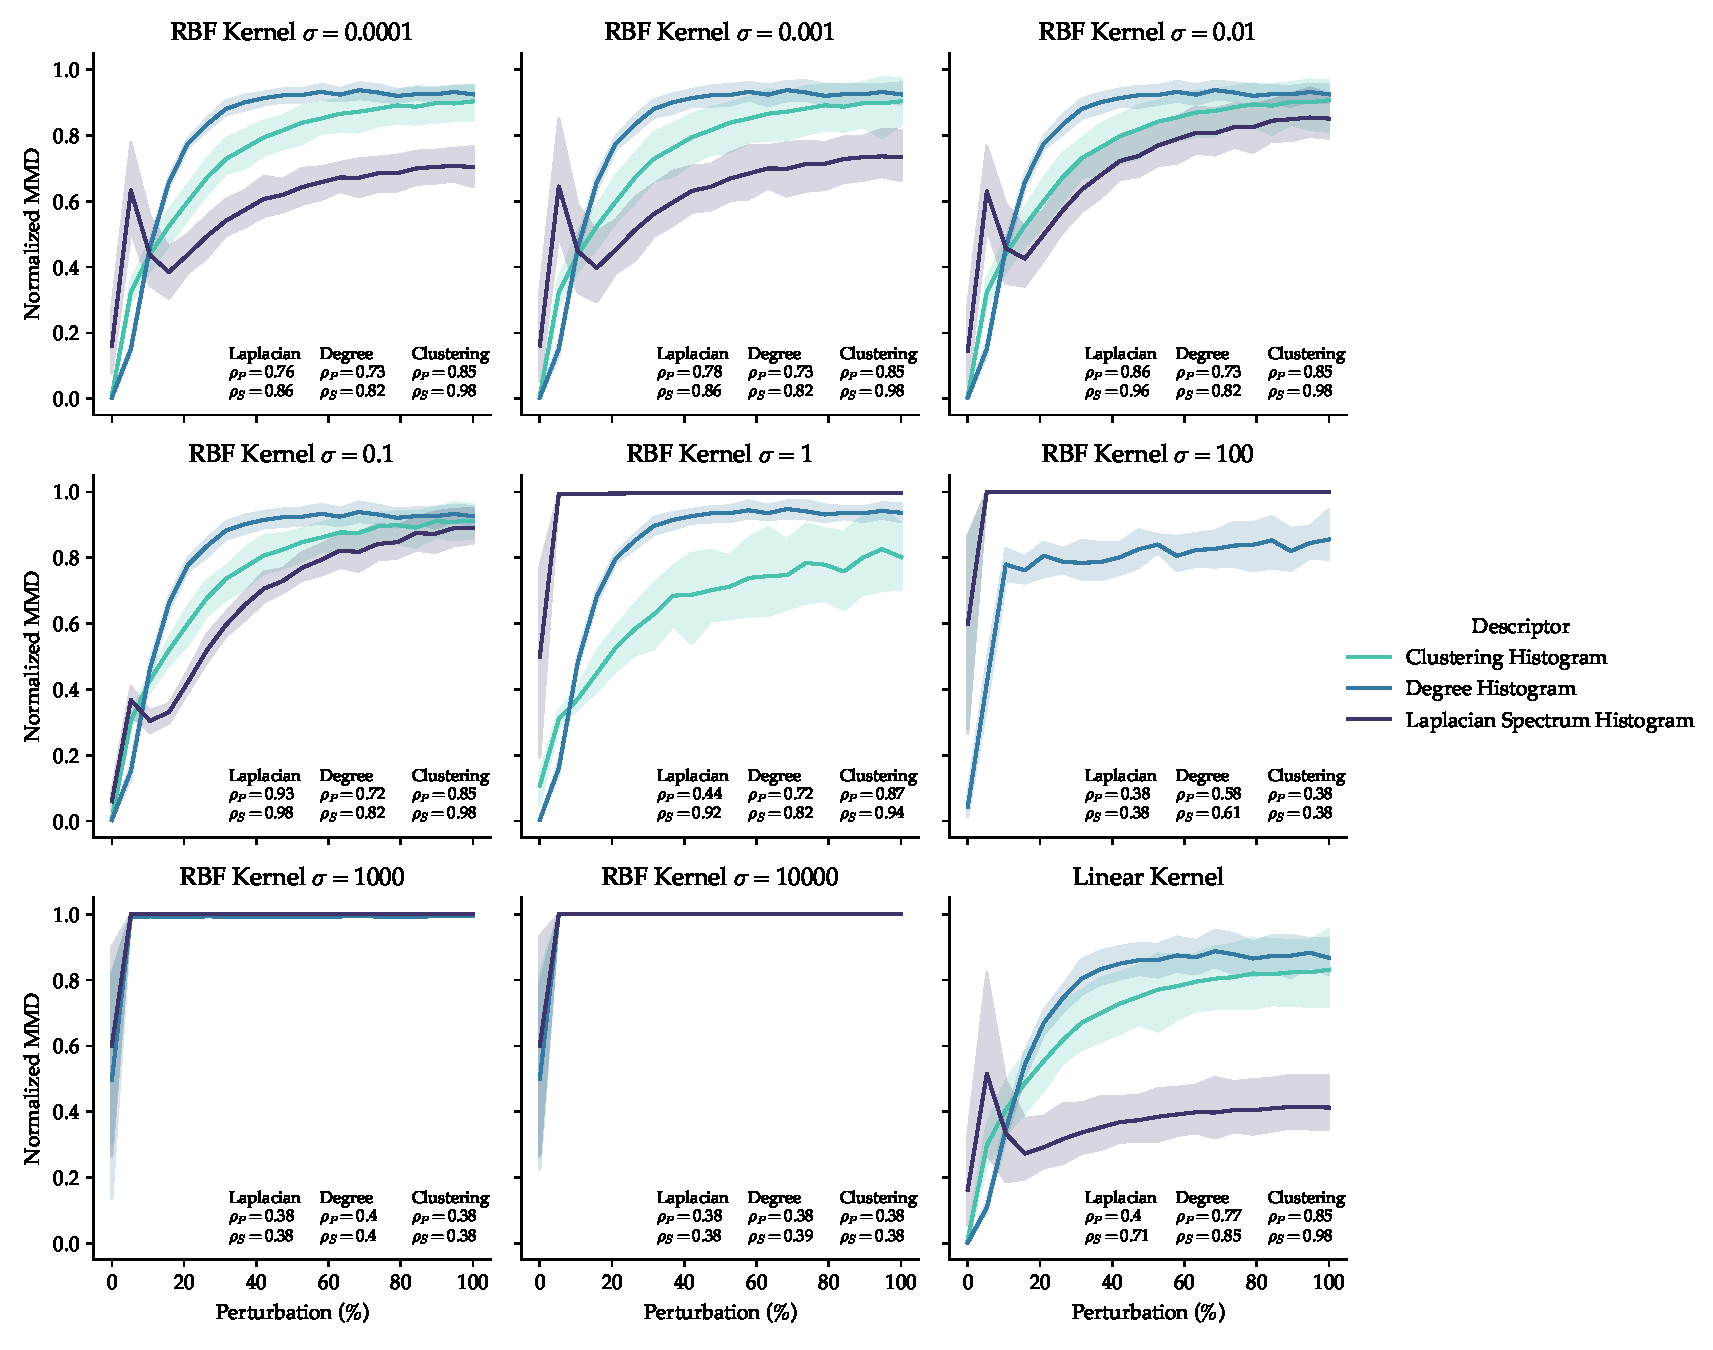
\includegraphics[width=\textwidth]{./figures/results/res_1_5.pdf}
  \caption[MMD vs. Gaussian Noise Perturbation (in \%) for various graph
descriptors of the 2-NN-graphs.]{MMD vs. Gaussian Noise Perturbation (in \%) for
various graph descriptors of the 2-NN-graphs. The kernel here is shown on top of
each subplots.}
  \label{fig:mmd_effect_kernel_knn}
\end{figure}


\section{Weisfeiler-Lehman Runtime Improvements for Sparse
  Graphs}\label{sec:sparse_wl}

In this thesis, we devised a three-pronged method to speed up the runtime of the
Weisfeiler-Lehman kernel by approximately 80\% by leveraging the sparsity of the
graphs used here. The three elements contributing to the speedup are the
following:

\begin{enumerate}
\item Our implementation parallelizes the execution of Weisfeiler-Lehman hash
computations since each graph's hash can be computed independently prior to
computing the kernel.
\item It also parallelizes the computation of similarity of graphs in RKHS by
computing batches of the inner products independently.
\item When comparing graphs, lots of CPU cycles are spent processing
positions/hashes that do not actually overlap between Weisfeiler-Lehman
histograms. As such, we manually loop over the overlapping keys, outperforming
numpy dot product-based implementations on collections of sparse graphs.
\end{enumerate}

We tested, covered, and open-sourced the implementation of this novel approach
on GitHub, and is available at the following URL: \url{https://github.com/pjhartout/fastwlk}.

\section{Distance Distribution of Descriptor Functions}
To explain why certain Gaussian configurations tend to work better than others,
it is useful to compute the pairwise distance of unperturbed proteins to get an
idea of how far away in e.g. Euclidean space, each embedding is from one
another.

\begin{figure}
  \centering
  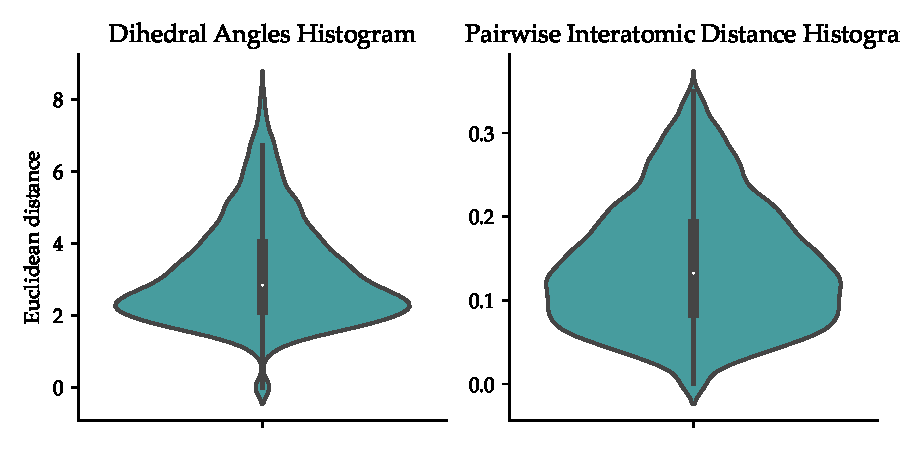
\includegraphics[width=0.6\textwidth]{./figures/results/violin_protein_descriptors.pdf}
  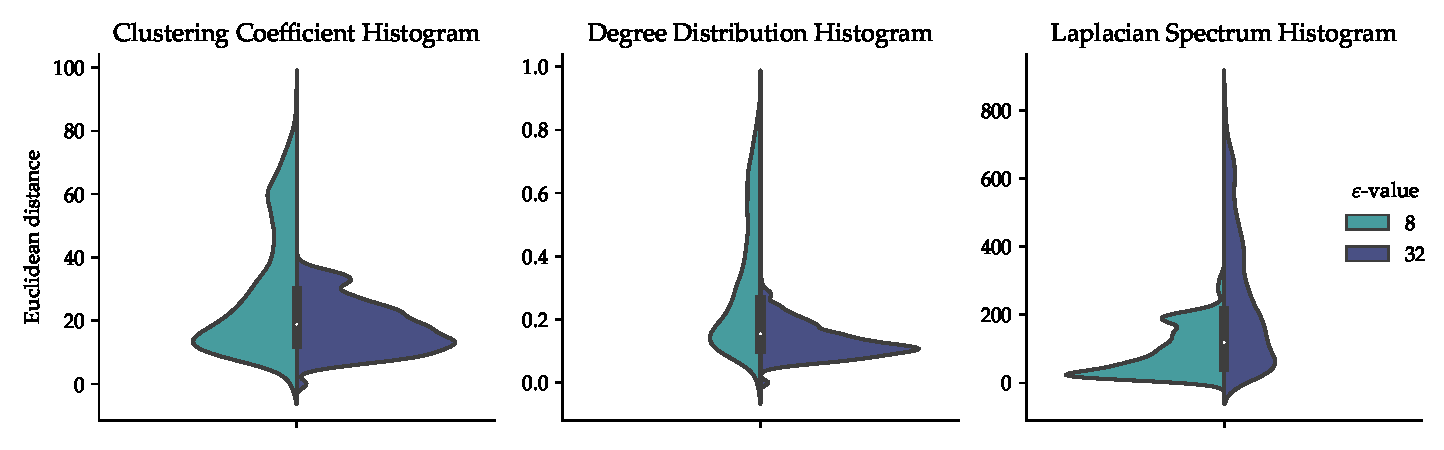
\includegraphics[width=\textwidth]{./figures/results/violin_graph_descriptors.pdf}
  \caption{Mean Euclidean distance between descriptor representations. The top
    row shows the mean distance between each of the protein descriptors
    introduced in this thesis while the bottom row shows the distance between
    each graph descriptor for two $\varepsilon$-graph extraction settings.}
\end{figure}


\backmatter

\bibliographystyle{plain}
\bibliography{refs}

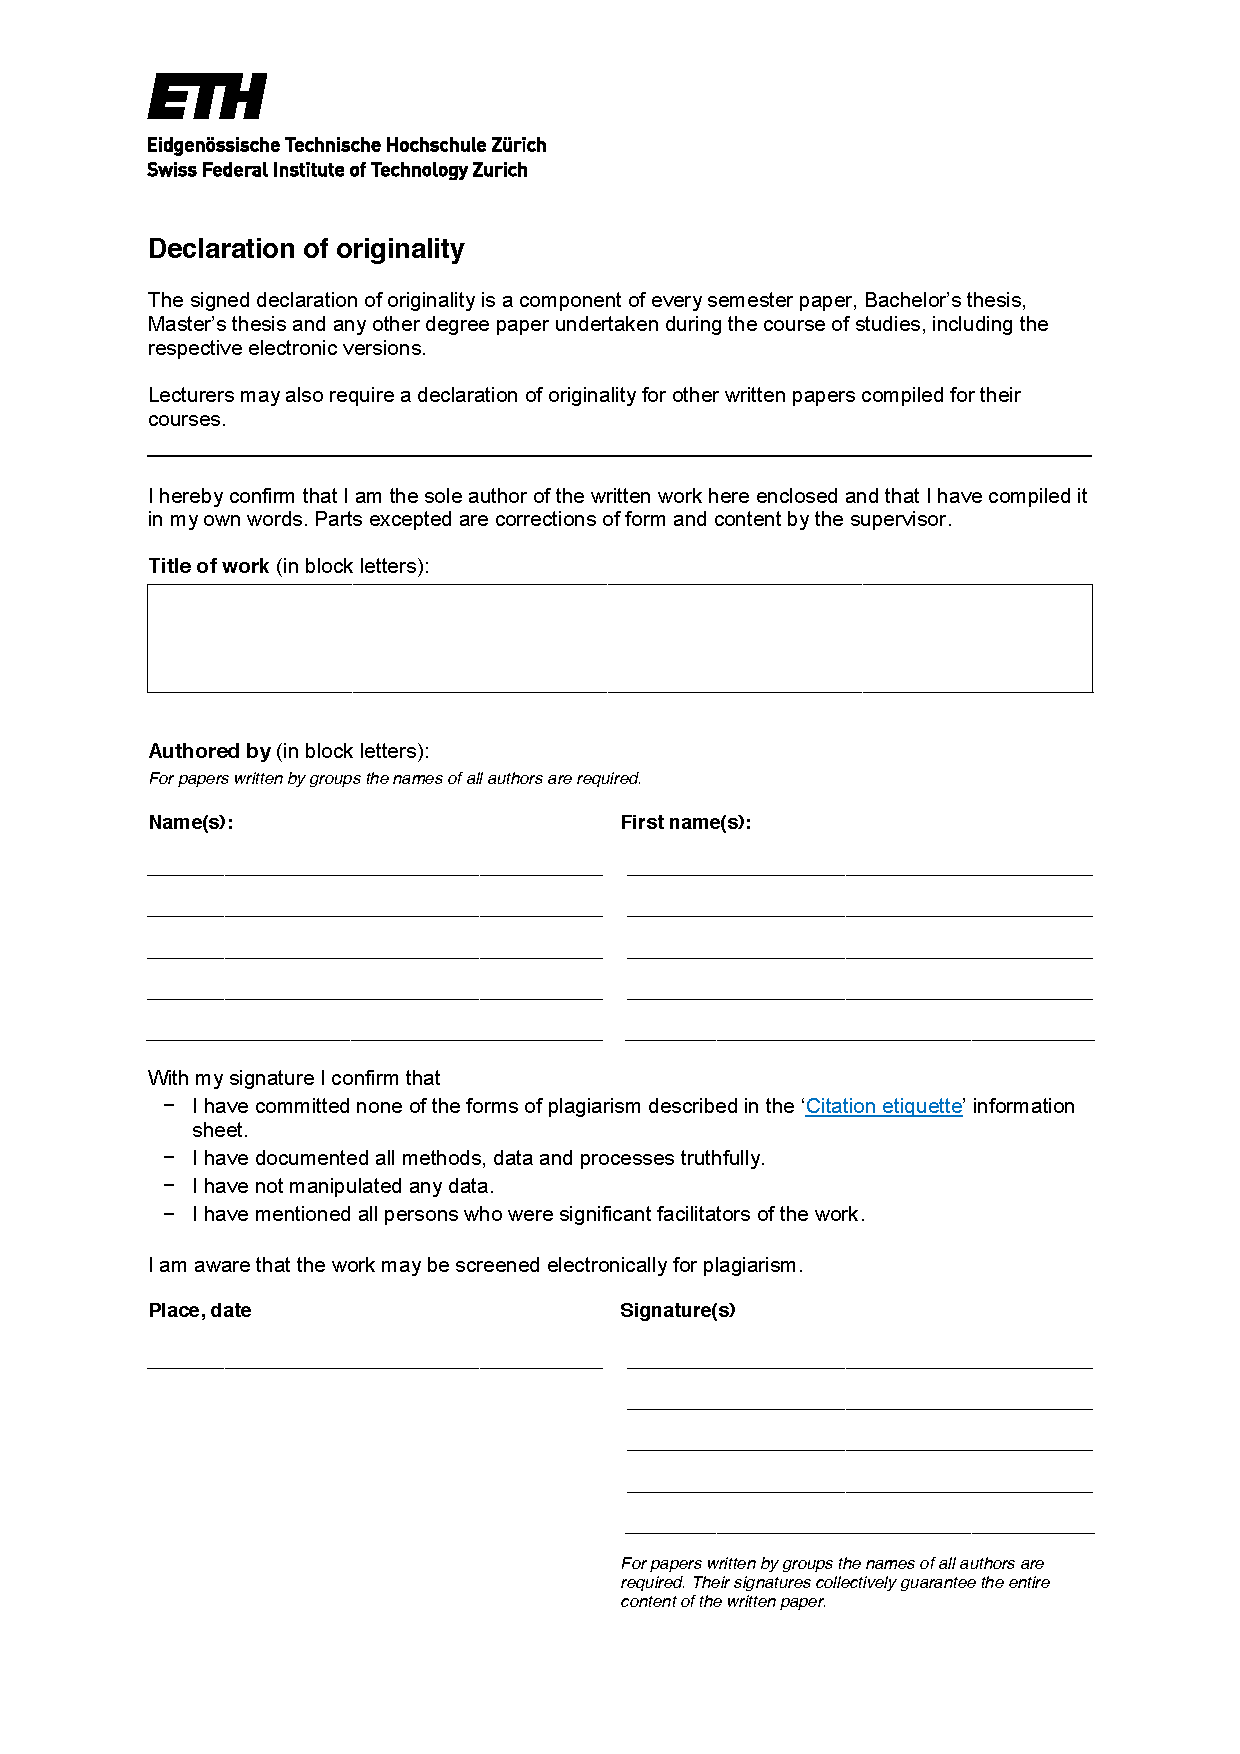
\includepdf[pages={-}]{declaration-originality.pdf}

\end{document}
